\title{\vspace{-2cm} \LARGE Divergence-Free Smoothed Particle Hydrodynamics \\ \large Advanced Simulation and Visualization of Fluids in Computer Graphics}

\author{\begin{tabular}{ccc}
    Isabell Jansson\thanks{isaja187@student.liu.se} & Ronja Grosz\thanks{rongr946@student.liu.se}  & Jonathan Bosson\thanks{jonbo665@student.liu.se}
\end{tabular}}

\date{\today}

\documentclass[11pt, twocolumn]{article}

% Our packages
\usepackage{graphicx}   % Images
\usepackage{amsmath}    % Math
\usepackage{amssymb}    % Math
\usepackage{listings}   % To write code in latex
\usepackage{color}      % Custom colors
\usepackage{abstract}   % Onecolabstract, saythanks
\usepackage[margin=1.2in]{geometry}

\usepackage{bm}
\newcommand{\vect}[1]{\bm{#1}} % bold vector

\setlength{\columnsep}{20px} % Length between twocolumn
 
\definecolor{codegreen}{rgb}{0,0.6,0}
\definecolor{codegray}{rgb}{0.5,0.5,0.5}
\definecolor{codepurple}{rgb}{0.58,0,0.82}
\definecolor{backcolour}{rgb}{0.95,0.95,0.92}

\lstdefinestyle{mystyle}{
    backgroundcolor=\color{backcolour},   
    commentstyle=\color{codegreen},
    keywordstyle=\color{magenta},
    numberstyle=\tiny\color{codegray},
    stringstyle=\color{codepurple},
    basicstyle=\footnotesize,
    breakatwhitespace=false,         
    breaklines=true,                 
    captionpos=b,                    
    keepspaces=true,                 
    numbers=left,                    
    numbersep=5pt,                  
    showspaces=false,                
    showstringspaces=false,
    showtabs=false,                  
    tabsize=2,
    literate={\ \ }{{\ }}1
}

\lstset{style=mystyle}
% END our packages

\begin{document}
\twocolumn[
\maketitle

\begin{onecolabstract}
    \noindent This paper discusses the technique presented by Bender et. al.~\cite{bender} for simulating incompressible fluids with an efficient and stable Divergence-Free Smoothed Particle Hydrodynamics method.
    The method uses two solvers to obtain a divergence-free fluid, a divergence solver and a density solver to correct the density after the divergence has been corrected.
    This results in a stable and fast simulation of a divergence-free fluid even though the simulation is performed on the CPU without any parallelization.
    \vspace{1em}\\{\bf Index Terms:} Incompressible fluids, Divergence-free, SPH, divergence correction, density correction.\vspace{1em}
\end{onecolabstract}
]
\saythanks

\section{Introduction}
    %explain the context of the work:
    %What exactly is the problem?
    %What have you created?
    Smoothed particle hydrodynamics, \textit{SPH}, is a method that was first implemented in 1977 for astrophysical simulations by Gingold et al.~\cite{firstSPH}.
    Since then SPH has become a popular method for complex fluid simulations.
    SPH is a mesh-free Lagrangian method where the fluid is split into discrete sets defined as particles, which move in space and change physical properties as time progresses.
    % More about Lagrangian and maybe navier stokes?
    
    % We used this article
    In this paper we are going to introduce the results from reproducing the divergence-free smoothed particle hydrodynamics method presented by Bender et al.~\cite{bender}.
    It is a method which corrects the divergence error, aiming for a divergence-free velocity field which is needed for an incompressible fluid.
    For the solution to be divergence-free the density has to be constant over time.
    
    % Write about other solutions? Why is this solution the BEST!!?

\section{Background and Related Work}
    %What have people done before?
    %When addressing this problem, when addressing similar problems
    %What have you done that makes you approach different?

    % Write about divergence free 
    In the field of computer graphics a variety of methods for simulating incompressible fluids exist.
    This section will give a brief overview of related approaches.

    Bender et al.~\cite{bender} proposed a method for a stable implicit SPH solution.
    The method uses a combination of two pressure solvers which enforce a low volume compression below 0.01$\%$ and a divergence-free velocity field.
    It can be seen as enforcing incompressibility on both position and velocity level.
    The low compression is important for realistic physical behavior and a divergence-free state increases the stability of the simulation which reduces the number of solver iterations.

    Another incompressible SPH method was proposed by Hu et al.~\cite{hu} for multiphase flows where the time integration step to obtain velocities is divided into two half steps.
    This is done to enforce both zero density variation condition and the velocity divergence-free condition at each full time step.
    During the first half step density fluctuations are eliminated by altering the intermediate particle position.
    During the second half step errors in velocity divergence are resolved by altering the intermediate particle velocity.

    Ihmsen et al.~\cite{ihmsen2014implicit} proposed an implicit incompressible SPH method with a pressure poisson equation made by the combination of a symmetric SPH pressure force and a SPH discretization of the continuity equation.
    The pressure poisson equation is used to compute the pressure so that the pressure forces correct the intermediate velocities to a divergence-free state.
    
    A predictive corrective incompressible SPH method was proposed by Solenthaler et al.~\cite{solenthaler} based on the Lagrangian SPH model.
    Incompressibility was enforced using a prediction correction scheme to determine the particle pressures.
    To achieve this the information about the density fluctuation was actively propagated through the fluid and the pressure values where updated until the targeted density was satisfied.

    A ghost fluid approach for free surface and solid boundary conditions for a SPH fluid simulation was proposed by Schechter et al.~\cite{ghost}.
    The ghost particles are placed on free surfaces and at solid boundary conditions.
    The approach solves problems like spurious numerical surface tension artifacts and errors in the mass conservation constraints.


\section{Method}
%What have you done?
%How did you do it?
%Why did you do it that way?
%May want to mention why you *didn’t* do it in some 
%other possible way
%Clear enough that you could hand the report to another student and they could reproduce the work!
%Probably no need to mention programming language etc

The produced simulation after following the method proposed by Bender et al.~\cite{bender} is drafted in Listing~\ref{lst:simulation}. 
Upon starting the application the particle neighbourhood $N_i$ will be determined with a cell list solution explained in Section~\ref{section:neighbour}.
For each particle the alpha $\alpha_i$ and density $\rho_i$ parameters will be computed, both of which are commonly reused variables and thus worth storing to reduce computation cost.
This is done before entering the simulation loop as initial values are required.
During the loop all these parameters will be updated as the simulation progresses.

Once in the simulation at line $7$ the first time step will be determined through the CFL condition explained in Section~\ref{section:timestep}.
The new velocities for each particle is then predicted through the included external forces which are propagated with ordinary Euler integration.

\begin{lstlisting}[caption={Simulation algorithm},label={lst:simulation}, language=C++, mathescape=true, escapeinside={(*}{*)}] 
function performFluidSimulation
    for all particles $i$ do //Init neighbourhoods
        find neighbourhoods $N_i(0)$
    for all particles $i$ do //Init $\color{codegreen}\rho_i$ and $\color{codegreen}\alpha_i$
        compute densities $\rho_i(0)$
        compute factors $\alpha_i(0)$
    while (t < $t_{max}$) do //Start simulation loop
        adapt time step $\Delta{t}$ 
        for all particles $i$ do //Predict velocities $\color{codegreen}\mathbf{v}_i^*$
            $\mathbf{v}_i = \mathbf{v}_i + \Delta{t}\mathbf{F}_g/m_i$
        correctDensityError($\alpha, \mathbf{v}_i$) //Fulfill $\color{codegreen}\rho^* - \rho_0 = 0$
        for all particles $i$ do //Update positions
            $x_i(t + \Delta{t}) = x_i(t) + \Delta{t}\mathbf{v}_i^*$
        for all particles $i$ do //Update neighbourhoods
            find neighbourhoods $N_i(t + \Delta{t})$
        for all particles $i$ do //Update $\color{codegreen}\rho_i$ and $\color{codegreen}\alpha_i$ 
            compute densities $\rho_i(0)$
            compute factors $\alpha_i(0)$
        correctDivergenceError($\alpha, \mathbf{v}^*$) //Fulfill $\color{codegreen}\frac{D\rho}{Dt} = 0$
\end{lstlisting}

The density solver uses the precomputed parameter $\alpha_i$ together with this prediction to compute the pressure forces in each neighbourhood such that it can correct the density error $\rho_i^* - \rho_i = 0$.
This is further explained in Section~\ref{densitySolver}.

After the particle position $\vect{x_i}$ has been updated the neighbourhoods and the $\alpha_i$ and $\rho_i$ factors are recalculated to reflect the new positions.
Lastly, in line $19$ of Listing~\ref{lst:simulation} the divergence solver, much like the density solver, calculates the pressure forces to eliminate its error.
In this case the divergence error $\frac{D\rho_i}{Dt}$ is corrected to be equal to $0$.

\subsection{Navier-Stokes}
    Navier-Stokes equations describe incompressible fluids and are therefore suitable for SPH simulations.
    The equations expressed in Lagrangian coordinates can be found in Equation~\ref{eq:nsDensity} and~\ref{eq:nsVelocity}.

    \begin{equation} \label{eq:nsDensity}
        \frac{D\rho}{Dt} = 0 \Leftrightarrow \nabla \cdot \textbf{v} = 0 
    \end{equation}

    \begin{equation} \label{eq:nsVelocity}
        \frac{D\textbf{v}}{Dt} = -\frac{1}{\rho} \nabla p + v \nabla ^2 \textbf{v} + \frac{\textbf{f}}{\rho}
    \end{equation}

    In the equations $\frac{D\rho}{Dt}$ and $\frac{D\textbf{v}}{Dt}$ denotes the derivate of the density $\rho$ and the velocity $\textbf{v}$ respectively.
    The pressure, kinematic viscosity and body forces are denoted by $p,v$ and $\textbf{f}$ respectively.
    The second part of Equation~\ref{eq:nsDensity}, $\nabla \cdot \textbf{v} = 0$, induce that the velocity field is free from divergence.
    From the continuity equation $\frac{D\rho}{Dt} = -\rho \nabla \cdot \textbf{v}$ and the divergence-free condition it follows that the partial derivate of the density with respect to the time is zero, which implies the equivalence of the equations in Equation~\ref{eq:nsDensity}.
    From this it follows that the density, in theory, must stay constant over time which is the implication of an incompressible fluid.
    In practice the divergence-free condition is not sufficient to guarantee incompressibility in simulations.
    The numerical time integrations will contain numerical errors which will cause density deviations due to the volume compressions.
    To avoid this a second condition $\rho - \rho_0 = 0$ called \textit{constant density condition} must be fullfilled~\cite{bender}.
    Section~\ref{densitySolver} and~\ref{divergenceSolver} give a deeper description of the solvers used in the project.


\subsection{Adapted time step} \label{section:timestep}

% CFL condition, explain why its necessary and how its assured that each rendered frame has the same time step.
In order to assure a stable simulation it is necessary to adapt the time step depending on the motion.
Depending on how quick the particles move, smaller time steps are taken such that the numerical error of the explicit time integration is negligible.
A condition was proposed by Courant$-$Friedrichs$-$Lewy, often refered to as the CFL-condition, which is shown in Equation~\ref{eq:cfl}.
The time step $\Delta t$ is equal to a fraction of the particle's diameter $d$ divided by 
the maximum velocity $\vect{V}_{max}$ in the scene.

\begin{equation} \label{eq:cfl}
\Delta t \leq \frac{0.4 \cdot d}{\vect{V}_{max}}
\end{equation}

Each rendered frame however have a constant time step in order to ensure no speed change in the playback of the rendered video.
This is decided from the user side as a desired fps parameter.
This means that the simulation loop can iterate multiple times within each frame adaptively depending on the maximum velocity of a particle.



\subsection{Neighbourhood search} \label{section:neighbour}
    Since SPH only considers a finite amount of neighbouring particles it is important to keep track of every particles' neighbours.
    Searching through all particles for neighbours within the cutoff distance $h$ for every particle is inefficient and takes $\mathcal{O}({N^2})$ time.
    The cutoff distance $h$ is the kernels' smoothing radius.
    To make this faster a cell list was implemented.
    A cell list is a data structure that is divided into cells that have a length larger or equals to the cutoff distance $h$.
    Each cell spans on a surface in space.
    A particle belongs to a cell if it is inside the space the cell occupy.
    When finding the neighbour of particle $i$, only the neighbouring cells have to be searched for particles within the cutoff distance, see Figure~\ref{fig:cellList}.
    
    \begin{figure}[h!]\centering
    \begin{centering}
    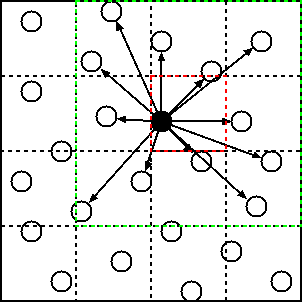
\includegraphics[width=0.7\linewidth]{img/CellList.png}
    \caption{Finding the neighbours for the filled in particle $i$ by looking through all neighbouring cells, including its own cell, for particles within the cutoff distance $h$}
    \label{fig:cellList}
    \end{centering}
    \end{figure}

    The cell list is implemented by using a four dimensional vector where the first three dimensions are for the $x$, $y$ and $z$ coordinates and the fourth dimension is for storing the index of the particles that belong to the cell.

    The amount of cells are decided by dividing the scene into cells of length $h$.
    The particles are then assigned to a cell by finding the cell's coordinates that it belongs to according to Equation~\ref{eq:assignCell}, where $\vect{x}$ is the position of the particle and $\vect{s}_{min}$ is the lowest position of the scene space.
    If the particle moves out of its cell it is reassigned to the new cell it is inside.

    \begin{equation} \label{eq:assignCell}
        \frac{\lceil{\vect{x} - \vect{s}_{min}}\rceil}{h}
    \end{equation}

% Should be mentioned early since it is used in mostly of the algorithms
\subsection{Kernel} \label{kernel}
    A kernel function is used to simulate how particle to particle interactions decrease with the distance between the current particle and its neighbours.
    In SPH simulations this is an approximation of the Gaussian kernel function.
    Different kernels have been tested in previous works i.e. the poly6 kernel, the spiky kernel and the cubic spline kernel.
    According to Bender et. al.~\cite{bender} the cubic spline kernel presented by Monaghan~\cite{monaghan} was used.
    The kernel is described by Equation~\ref{eq:kernel}, where $q(x)=\frac{\left \| x \right \|}{h}$, $x$ is the distance between the current particle and a neighbour particle and $h$ is the support radius for the kernel.
    Particles further away than the support radius will not affect the current particle.

    \begin{equation} \label{eq:kernel}
        \resizebox{0.88\linewidth}{!}{$
        W_h(q(x)) =  \frac{1}{\pi h^3} \left\{\begin{matrix}
        1 - \frac{3}{2}q^2 + \frac{3}{4}q^3 & 0 \leqslant q < 1 \\ 
        \\
        \frac{1}{4}(2-q)^3 & 1 \leqslant q < 2\\ 
        \\
        0 & q \geqslant 2
        \end{matrix}\right.
        $}
    \end{equation}

    The algorithm does also require the kernel gradient.
    To reduce the computational effort and memory requirements Bender et. al.~\cite{bender} introduce a scalar function $g(q) = \frac{\partial W_h}{\partial q} \cdot \frac{1}{h \left \| x \right \|}$.
    The gradient kernel is then calculated by $\partial W_h(q(x)) = x \cdot g(x)$.
    The gradient kernel is described by Equation~\ref{eq:gradKernel}.


    \begin{equation} \label{eq:gradKernel}
        \resizebox{0.88\linewidth}{!}{$
        \partial W_h(q(x)) =  x \frac{1}{h \left \| x \right \|} \frac{1}{\pi h^3} \left\{\begin{matrix}
        - 3q + \frac{9}{4}q^2 & 0 \leqslant q < 1 \\ 
        \\
        - \frac{3}{4}(2-q)^2 & 1 \leqslant q < 2\\ 
        \\
        0 & q \geqslant 2
        \end{matrix}\right.
        $}
    \end{equation}
    % maybe specify x here as well 

    It is important to use the same kernel function for both $W_h$ and $\nabla W_h$ to get the prediction and the correction step to be compatible to each other.


\subsection{Density and alpha factors} \label{section:alpha}
    The density in a region of the fluid with a particle $x_i$ in the center is calculated through Equation~\ref{eq:density} where $\rho_i$ is the density with the current particle $x_i$ in center, $\rho_j$ is the density with a neighbouring particle $x_j$ in center, $m_j$ is the mass for a neighbour particle and $W_{ij}$ is the kernel function described in Section~\ref{kernel}.
    This implies that neighbouring particles closer to the current particle $x_i$ will have a greater affect on the density.

    \begin{equation} \label{eq:density}
        \rho_i = \sum_j \frac{m_j}{\rho_j} \rho_j W_{ij} = \sum_j m_j W_{ij}
    \end{equation} 

    Both the density solver and the divergence solver uses a stiffness parameter $\kappa_i^v$ presented by Bender et. al.~\cite{bender}, Equation~\ref{eq:kappa}.

    \begin{equation} \label{eq:kappa}
        \kappa_i^v = \frac{1}{\Delta t} \frac{D\rho_i}{Dt} \cdot \alpha_i
    \end{equation} 

    In the equation $\Delta t$ denotes a small time step and $\alpha_i$ is a precomputed factor to decrease the computations while performing the solvers.
    Bender et. al.~\cite{bender} defines $\alpha_i$ as

    \begin{equation} \label{eq:alpha}
        \alpha_i = \frac{\rho_i}{\left | \sum_j m_j \nabla \vect{W}_{ij}  \right |^2 + \sum_j \left | m_j \nabla \vect{W}_{ij} \right |^2}
    \end{equation}

    where $\vect{W}_{ij}$ corresponds to the kernel gradient.

\subsection{Density solver} \label{densitySolver}
    This solver aims to minimize the density error caused by the numerical integration in the divergence solver.
    The density error is determined by comparing the actual density to the rest density, $\rho - \rho_0$.
    There are several density solvers presented in previous works, but the solver used in this project was presented by Bender et. al.~\cite{bender} which uses the fact that $\alpha_i$ has been calculated before the solver which reduces the computations in the solver.
    The solver will be active while the average of the predicted densities for every particle differs from the rest density with an error greater than a constant \textit{maxError}.
    For every particle a predicted density $\rho_i^*$ is calculated through an Euler integration step by Equation~\ref{eq:predDensity}.

    \begin{equation} \label{eq:predDensity}
        \resizebox{0.85\linewidth}{!}{$
        \begin{matrix}
        \rho_i^* = \rho_i + \Delta t \frac{D\rho_i}{Dt} \\ 
        \\
        \Leftrightarrow \\ 
        \\
        \rho_i^* = \rho_i + \Delta t \sum_j m_j 
        (\textbf{v}_{i}^* - \textbf{v}_j^*) \nabla \vect{W}_{ij}
        \end{matrix}
        $}
    \end{equation}


    \begin{equation} \label{eq:pressure}
        \vect{F_i^p} = -\frac{m_i}{\rho_i}\nabla \vect{p_i}
    \end{equation}

    The pressure force of a particle is determined by Equation~\ref{eq:pressure}, where the pressure gradient can be solved using the SPH formulation proposed by Ihmsen et al.~\cite{ihmsen}, Equation~\ref{eq:pressureGrad}.

    \begin{equation} \label{eq:pressureGrad}
        \nabla \vect{p_i} = \kappa_i^v \nabla \rho_i = \kappa_i^v \sum_j m_j \nabla \vect{W_{ij}}
    \end{equation}

    \begin{equation} \label{eq:pressure2}
        \vect{F_{j\leftarrow i}^p} = -\frac{m_i}{\rho_i} \kappa_i^v m_j \nabla \vect{W}_{ij}
    \end{equation}

    Further on, the pressure forces $\vect{F_{j\leftarrow i}^p} $ that act from particle $i$ on all its neighbours $j$ is calculated through Equation~\ref{eq:pressure2}, where the stiffness parameter $\kappa_i$ is determined by Equation~\ref{stiffnessDensity}.

    \begin{equation} \label{stiffnessDensity}
    \kappa_i = \frac{1}{\Delta t^2}(\rho_i^*-\rho_0)\alpha_i
    \end{equation}

    To conserve momentum it is required that all inner pressure forces sum up to zero such that $\vect{F_i^p} + \vect{F_{j\leftarrow i}^p} = 0$.
    As proposed by Bender et. al~\cite{bender} the solver computes the total force $\vect{F_{i,total}^p}$ through Equation~\ref{eq:pressureTotal}.

    \begin{equation} \label{eq:pressureTotal}
        \resizebox{0.85\linewidth}{!}{$
        \begin{matrix}
            \vect{F_{i,total}^p} = \vect{F_i^p} + \sum_j \vect{F_{i\leftarrow j}^p} \\
            \\
            \Leftrightarrow \\ 
            \\
            \vect{F_{i,total}^p} = -m_i \sum_j m_j (\frac{\kappa_i^v}{\rho_i} + \frac{\kappa_j^v}{\rho_i}) \nabla \vect{W}_{ij}
        \end{matrix}
        $}
    \end{equation}

    Newton's second law $F = ma = m\frac{dv}{dt}$ implies that $\frac{dv}{dt}$ is according to Equation~\ref{dvdt}. 
    The velocity of particle $i$ is thus changed according to Equation~\ref{eq:velocity}.

    \begin{equation} \label{dvdt}
        \frac{dv}{dt} = \sum_j m_j (\frac{\kappa_i^v}{\rho_i} + \frac{\kappa_j^v}{\rho_i}) \nabla \vect{W}_{ij}
    \end{equation}


    \begin{equation} \label{eq:velocity}
        \resizebox{0.85\linewidth}{!}{$
        \vect{v_{i+1}^*}(t) = \vect{v_i^*}(t) - \Delta t \sum_j m_j (\frac{\kappa_i^v}{\rho_i} + \frac{\kappa_j^v}{\rho_i}) \nabla \vect{W}_{ij}
        $}
    \end{equation}

% Write about non pressure forces, velocity osv..?


\subsection{Divergence solver} \label{divergenceSolver}

    \iffalse
    \begin{lstlisting}[language=C++, mathescape=true, escapeinside={(*}{*)}]
        function correctDivergenceError
            for all particles $i$ do
                calculateDensityChange $\frac{Dp}{Dt}_i$
            for all particles $i$ do //Scale $\color{codegreen}a_i$
                $a_i = \frac{a_i}{\Delta t}$
            while (t < $t_{max}$) do //Start simulation loop
                adapt time step $\Delta{t}$ 
                for all particles $i$ do //Predict velocities $\color{codegreen}\mathbf{v}_i^*$
                    $\mathbf{v}_i = \mathbf{v}_i + \Delta{t}\mathbf{F}_i^{adv}/m_i$
                correctDensityError($\alpha, \mathbf{v}_i$) //Fulfill $\color{codegreen}\rho^* - \rho_0 = 0$
                for all particles $i$ do //Update positions
                    $x_i(t + \Delta{t}) = x_i(t) + \Delta{t}\mathbf{v}_i^*$
                for all particles $i$ do //Update neighbourhoods
                    find neighbourhoods $N_i(t + \Delta{t})$
                for all particles $i$ do //Update $\color{codegreen}\rho_i$ and $\color{codegreen}\alpha_i$ 
                    compute densities $\rho_i(0)$
                    compute factors $\alpha_i(0)$
                correctDivergenceError($\alpha, \mathbf{v}^*$) //Fulfill $\color{codegreen}\frac{D\rho}{Dt} = 0$
        \end{lstlisting}
    \fi

    The divergence-free solver ensures the fluid to be free of density change over time by enforcing $\frac{D\rho}{Dt} = 0$, which is equivalent to the Navier-Stokes divergence free condition given in Equation~\ref{eq:nsDensity}.
    \\ \\ Equation~\ref{eq:dpdt} defines how the density change is computed.
    As in the density solver, the total pressure forces acting on a particle $i$ are computed.
    The stiffness parameter is calculated through Equation~\ref{eq:kappaDivergence}.

    \begin{equation} \label{eq:dpdt}
        \frac{D\rho_i}{Dt} = \sum_j m_j (\vect{v_i} - \vect{v_j})\nabla \vect{W}_{ij}
    \end{equation}

    \begin{equation}\label{eq:kappaDivergence}
        \kappa_i^v = \frac{1}{\Delta t} \frac{D\rho_i}{Dt} \cdot \alpha_i
    \end{equation}


    The stiffness parameters need to be determined iteratively since neighboring particles depend on each other.
    After the symmetric pressure force has been applied to the new velocity should the density change in Equation~\ref{eq:dpdt} be equal or close to zero.
    If the error is too large the process will be iterated until desired result have been achieved.


\subsection{Boundary conditions}
Dirichlet boundary condition was implemented in order to simulate the fluid inside a bounding box.
Dirichlet assumes that the pressure is zero outside the fluid and therefore the value a quantity has to take along the boundary has to be specified, in this case the velocity was set to zero when a particle reaches the boundary, Bridson~\cite{bridson}.

An isosurface was also introduced in the middle of the scene in order to simulate collisions with arbitrary objects.
This was done as an implicit representation of geometric shapes, described as a function $f(x,y,z)$.
Given an isovalue $C = f(\vect{x})$, point $\vect{x}$ can be classified as follows:

\begin{eqnarray} \label{eq:classifications}
\begin{array}{ll}
 \mbox{Inside:} & f(\mathbf{x}) < C \\
 \mbox{Outside:} & f(\mathbf{x}) > C \\
 \mbox{On surface:} & f(\mathbf{x}) = C \\  
  \end{array}
\end{eqnarray}

All possible implicit geomitries can be descibed by a quadratic function, which is found in Equation~\ref{eqn:quadratic}, and in matrix form in Equation~\ref{eqn:quadricmatrixform}.

\begin{eqnarray}
\label{eqn:quadratic}
f(x,y,z) &=
\nonumber & Ax^2+2Bxy+2Cxz\\
 &+&2Dx+Ey^2+2Fyz\\
\nonumber &+&2Gy+Hz^2+2Iz\\
\nonumber &+&J
\end{eqnarray}

\begin{eqnarray} \label{eqn:quadricmatrixform}
\resizebox{0.9\linewidth}{!}{$
\mathbf{p}^T\mathbf{Q}\mathbf{p} =  \left[ \begin{array}{cccc} x & y & z & 1 \end{array} \right] \left[ \begin{array}{cccc}
A & B & C &D\\
B & E & F & G\\
C & F & H & I\\
D & G & I & J\\
 \end{array} \right] \left[ \begin{array}{c}x \\
y \\
z \\
1 \end{array} \right]
$}
\end{eqnarray}

Considering that the geometry is placed at the origin, $f(\vect{x}) = 0$ means the particle is on the surface and $\vect{p}^T\vect{Q}\vect{p} \leq 0$ can be used to determine collisions.

Since the quadric surface is known analytically the differentiation can be applied to the quadric directly to get the gradient of the shape in position $\vect{x}$.
This gives an efficient and analytical expression with a coefficient matrix $Q$, which is used to help determine the new velocity direction of a particle after colliding with the surface.

\begin{eqnarray} \label{eq:quadricnormal}
\nabla f(x,y,z) = 2 \left[ \begin{array}{cccc}
A & B & C &D\\
B & E & F & G\\
C & F & H & I\\
 \end{array} \right] \left[ \begin{array}{c}x \\
y \\
z \\
1 \end{array} \right]\\
\nonumber = 2\mathbf{Q}_{sub}\mathbf{p}
\end{eqnarray} 

\section{Implementation}
%Details of how it was done
%What hardware
%What software
%Why did you do it that way?
%What limitations, if any, did this present?
%*No code*!!!!!
    % Talk about what we used for plugins, computers etc maybe or should this be in method?

    % Libraries
    % Computers
    % OpenGL
    % language
    % Makefiles
    The divergence-free SPH simulation was developed using OpenGL and C++ together with the OpenGL mathematics library GLM for vector calculations.
    FreeImage was used to save frames of the simulation and FFmpeg to assembled the frames into a video.
    PicoJSON was used to load in variables from a file making it easier to change variables quick and efficient and a makefile was used to compile the project.

    The simulation was developed on macOS and Linux.
    The Linux computer is running on Debian and has four Intel(R) Core(TM) i5-2450M CPU @ 2.50GHz, one NVIDIA GeForce 610M graphics card and 6.0 GiB RAM.
    One of the Mac OS computer is running on macOS Sierra and has a 1.8 GHz Intel Core i5 processor with an Intel HD Graphics 400 1536 MB graphics card.


\section{Results}
%What is the end product:
%What does it look like?
%How does one control and interact with it?
%How quick is it?
%What limitations does it have?
%Be self-critical and honest about it - or I will be

	When the application starts, the water is represented as set of spheres where every sphere has the properties of a particle.
	The initial state is illustrated in Figure~\ref{fig:res1}
	The water is affected by a gravity which induce a falling motion, illustrated in Figure~\ref{fig:res2}.

	\begin{figure}[h!]
		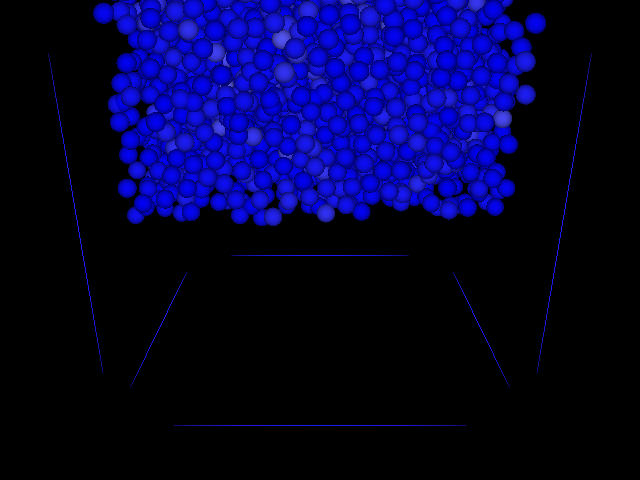
\includegraphics[width=\linewidth]{img/frame0001.png}
		\caption{Inital state of the water when the application starts.}
		\label{fig:res1}
	\end{figure}

	\begin{figure}[h!]
		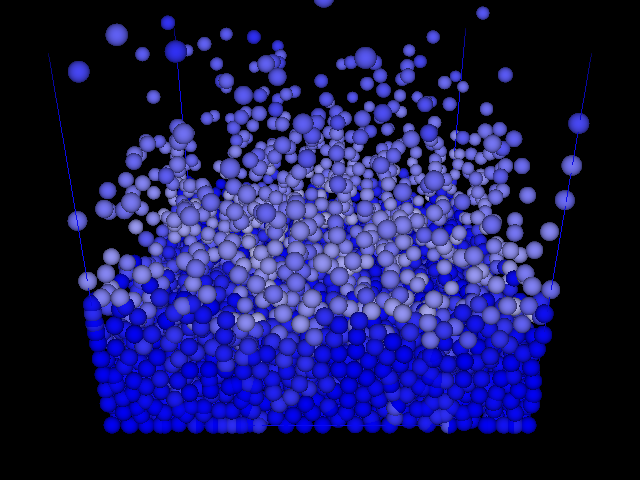
\includegraphics[width=\linewidth]{img/frame0139.png}
		\caption{The water falls due to the gravity.}
		\label{fig:res2}
	\end{figure}

	Since the water aims to be in the state of rest, the motion will decrease over time which is illustrated in Figure~\ref{fig:res3}.
	\begin{figure}[h!]
		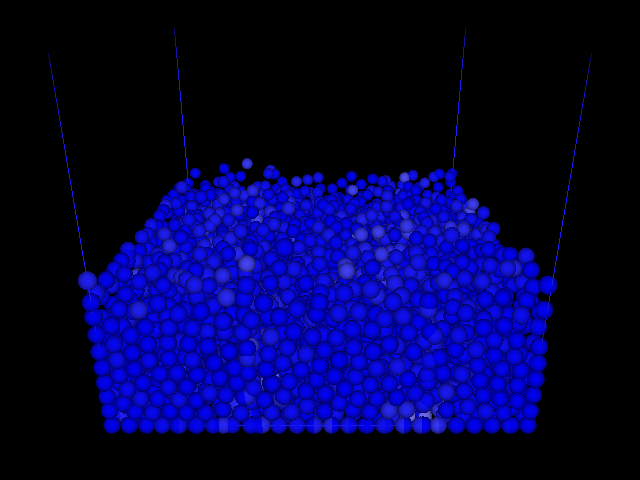
\includegraphics[width=\linewidth]{img/frame0500.png}
		\caption{The water is calm with some motion.}
		\label{fig:res3}
	\end{figure}

	To be able to simulate how outer forces affect the water, we implemented a feature where the user is able to change the direction of the force
	The result when applying a force from right to left on the water and then letting only the gravity affect it is shown in Figure~\ref{fig:res4}.

	\begin{figure}[h!]
		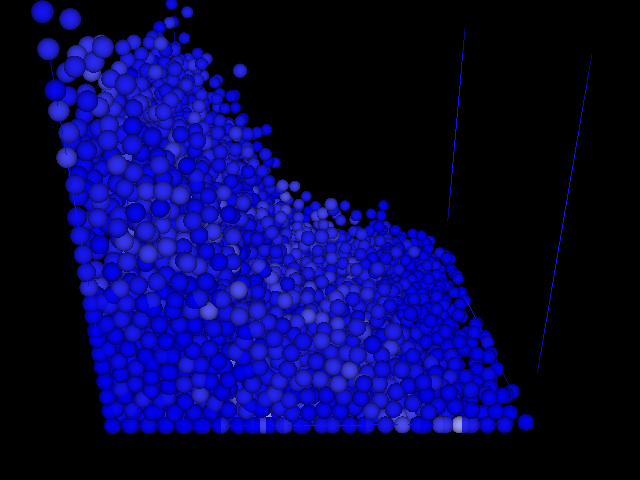
\includegraphics[width=\linewidth]{img/frame0882.png}
		\caption{The water after an applied right to left motion followed by gravity as the only outer force.}
		\label{fig:res4}
	\end{figure}

    % Results from adding cylinder

    % Write about FPS when running x amount of particles
	When running the program in real time with 5000 particles it runs with a frame rate of 6-8 fps on the MAC computer.
	When instead simulating with $10,000$ particles the frame rate is about 2 fps on the MAC computer.

\section{Conclusions and Future Work}
%Based on the results and evaluation
%Say what you’ve done right... ...and what you’ve done wrong! - be honest!
%Suggest some possible ways that the work could have been done better
%Suggest some ways that it could be extended and improved by adding more effort

    % Use ghost-SPH or similar
    To increase the accuracy of the interaction with the boundary and free surfaces a method like ghost-SPH that was presented by Schechter et al.~\cite{ghost} could be implemented.
    A method that Bender et al.~\cite{bender} used was the versatile rigid fluid coupling method for incompressible SPH presented by Akinci et al.~\cite{akinci2012versatile}.
    It is based on static boundary particles which could also be a valid implementation to get better boundary interactions.

    % Parallelize 
    To get the simulation to be able to handle more particles the solution could be parallelized to speed up the calculations.
    This could be done using OpenMP and increasing the threading.

    % Viscosity
    To get the simulation more interesting viscosity can be introduced into the fluid simulation.
    It would make simulations of thicker fluids possible.

    % Look up table for kernel values
    According to Bender et al.~\cite{bender} the kernel values could easily be precomputed and used together with a look up-table in order to speed up the calculations. This will result in a $30\%$ faster application.  This could be done once when the iteration loop begins and the positions for the particles are determined. Another approach would be to compute a discrete representation of the kernel function before the iteration loop and interpolate between to kernel values in the simulation loop in order to find a kernel value for a specific particle. 

\bibliographystyle{ieeetr}
\bibliography{./refs}

\end{document}
